\documentclass[12pt]{article}
 
\usepackage[margin=1in]{geometry}
\usepackage[font=small,labelfont=bf]{caption}
\usepackage{graphicx}
%\usepackage[draft]{graphicx}
\usepackage{amsmath, amsthm, amssymb, bm, enumitem, nicefrac, float, booktabs, adjustbox, subcaption, fancyhdr, makecell, titlesec, dsfont, epigraph}
\PassOptionsToPackage{hyphens}{url}\usepackage{hyperref}

\newcommand{\N}{\mathbb{N}}
\newcommand{\Z}{\mathbb{Z}}
\DeclareMathOperator*{\argmax}{argmax}
%\DeclareMathOperator*{\argmin}{argmin}
\newcommand{\argmin}{\mathop{\mathrm{argmin}}} 
\setcounter{MaxMatrixCols}{20}


\pagestyle{fancy}
\fancyhead{}
\setlength{\headheight}{15pt}
\setlength{\emergencystretch}{2pt} 
\fancyfoot{}
\fancyhead[L]{\slshape{Daily Fantasy Football}}
\fancyhead[R]{\slshape J.R. Becker \& J. St. Clair}
\fancyfoot[C]{\thepage}


\begin{document}

\begin{titlepage}
	\begin{center}
	\vspace*{4cm}
	\huge{\textbf{Daily Fantasy Football}}\\[2cm]
	\Large{By\\[2mm] Jason R. Becker \& Jack St. Clair}\\[2cm]
	\large{A report submitted as an independent study project for the\\
		Master of Financial Engineering Program at the\\
		 University of California, Berkeley}\\[1cm]	
	\Large{Spring 2019}\\[2cm]
	
\includegraphics[scale=0.3]{../figures/fantasy_logo}
	\vfill
	\line(1,0){400}
	\end{center}
\end{titlepage}


\section{Introduction}
TODO



\pagebreak
\section{Data Summary}
TODO


\subsection{Data Collection}
\begin{table}[H]
\caption{Data collected from each source.}
\small
\label{sources}
\centering
\begin{tabular}{lcc}
	\toprule
	Source        &  Full Season              &  Weekly \\
	\midrule
	CBS           &  QB, RB, WR, TE, DST, K   &   QB, RB, WR, TE, DST, K \\
	ESPN          &  QB, RB, WR, TE, DST, K   &   QB, RB, WR, TE, DST, K \\
	FantasyPros   &  QB, RB, WR, TE, DST, K   &   QB, RB, WR, TE, DST, K \\
	FFToday       &  QB, RB, WR, TE, DST, K   &   QB, RB, WR, TE, K \\
	NFL.com       &  QB, RB, WR, TE, DST, K   &   QB, RB, WR, TE, DST, K \\
	RTSports      &  QB, RB, WR, TE, DST, K   &    {} \\
	Yahoo         &  {}                       &   QB, RB, WR, TE, DST, K \\
	\midrule
	DraftKings    &  {}                       &   QB, RB, WR, TE, DST \\
 	FanDuel       &  {}                       &   QB, RB, WR, TE, DST \\
	\bottomrule
\end{tabular}
\end{table}

For the scope of this report, full season analysis will be neglected. However, the data has been collected, allowing for potential future work on full season projections which may prove useful for season long fantasy leagues. As daily fantasy websites such as DraftKings and FanDuel do not include kickers in possible lineups, kickers will also be neglected for the remainder of this report.\bigskip

For each position, a variety of stats are projected from the various sources. Due to lack of consistency between which stats are projected and which are not among the sources, stats were broken down into two categories. The first category we denote \textit{essential stats}, stats which are projected by most of the sources and are generally non-zero in value. The second category we denote \textit{nonessential stats}, stats which may not be projected by more than a couple sources and are generally 0 or near 0 in value. Table \ref{stats table} lists the essential and nonessential stats for each position.

\begin{table}[H]
\caption{Essential and nonessential stats for each position.}
\small
\label{stats table}
\centering
\begin{adjustbox}{width =\textwidth}
\begin{tabular}{lcc}
	\toprule
	Position        &  Essential Stats            &  Nonessential Stats \\
	\midrule
	QB   &  Pass Yds, Pass TD, Pass Int, Rush Yds, Rush TD,   &   Receptions, Rec Yds, Rec TD, 2PT\\
	RB   &  Rush Yds, Rush TD, Receptions, Rec Yds, Rec TD   &   Pass Yds, Pass TD, Pass Int, 2PT \\
	WR   &  Rush Yds, Rush TD, Receptions, Rec Yds, Rec TD   &   Pass Yds, Pass TD, Pass Int, 2PT \\
	TE   &  Receptions, Rec Yds, Rec TD    &   Pass Yds, Pass TD, Pass Int, Rush Yds, Rush TD, 2PT\\
	DST  &  PA, YdA, TD, Sack, Int, Fum Rec & Saf, Blk \\
	\bottomrule
\end{tabular}
\end{adjustbox}
\end{table}


\subsection{Missing Data}

Among data collection sources, the number of players with projections was not consistent, and in many cases projections are only provided from 4 or 5 out of 6 sources for a particular player. The number of sources which provided projections for each essential stat, and the percentage of missing data are provided in Figure \ref{missing data}. Nonessential statistics are provided in the appendix. These instances were manually observed and found to not be restricted to backups, but often occur in prominent starting players (e.g., Drew Brees, Cam Newton). Since prominent players were affected, the players with missing projections could not be dropped, necessitating imputing of missing values.\bigskip


\begin{figure}[H]
  \centering
  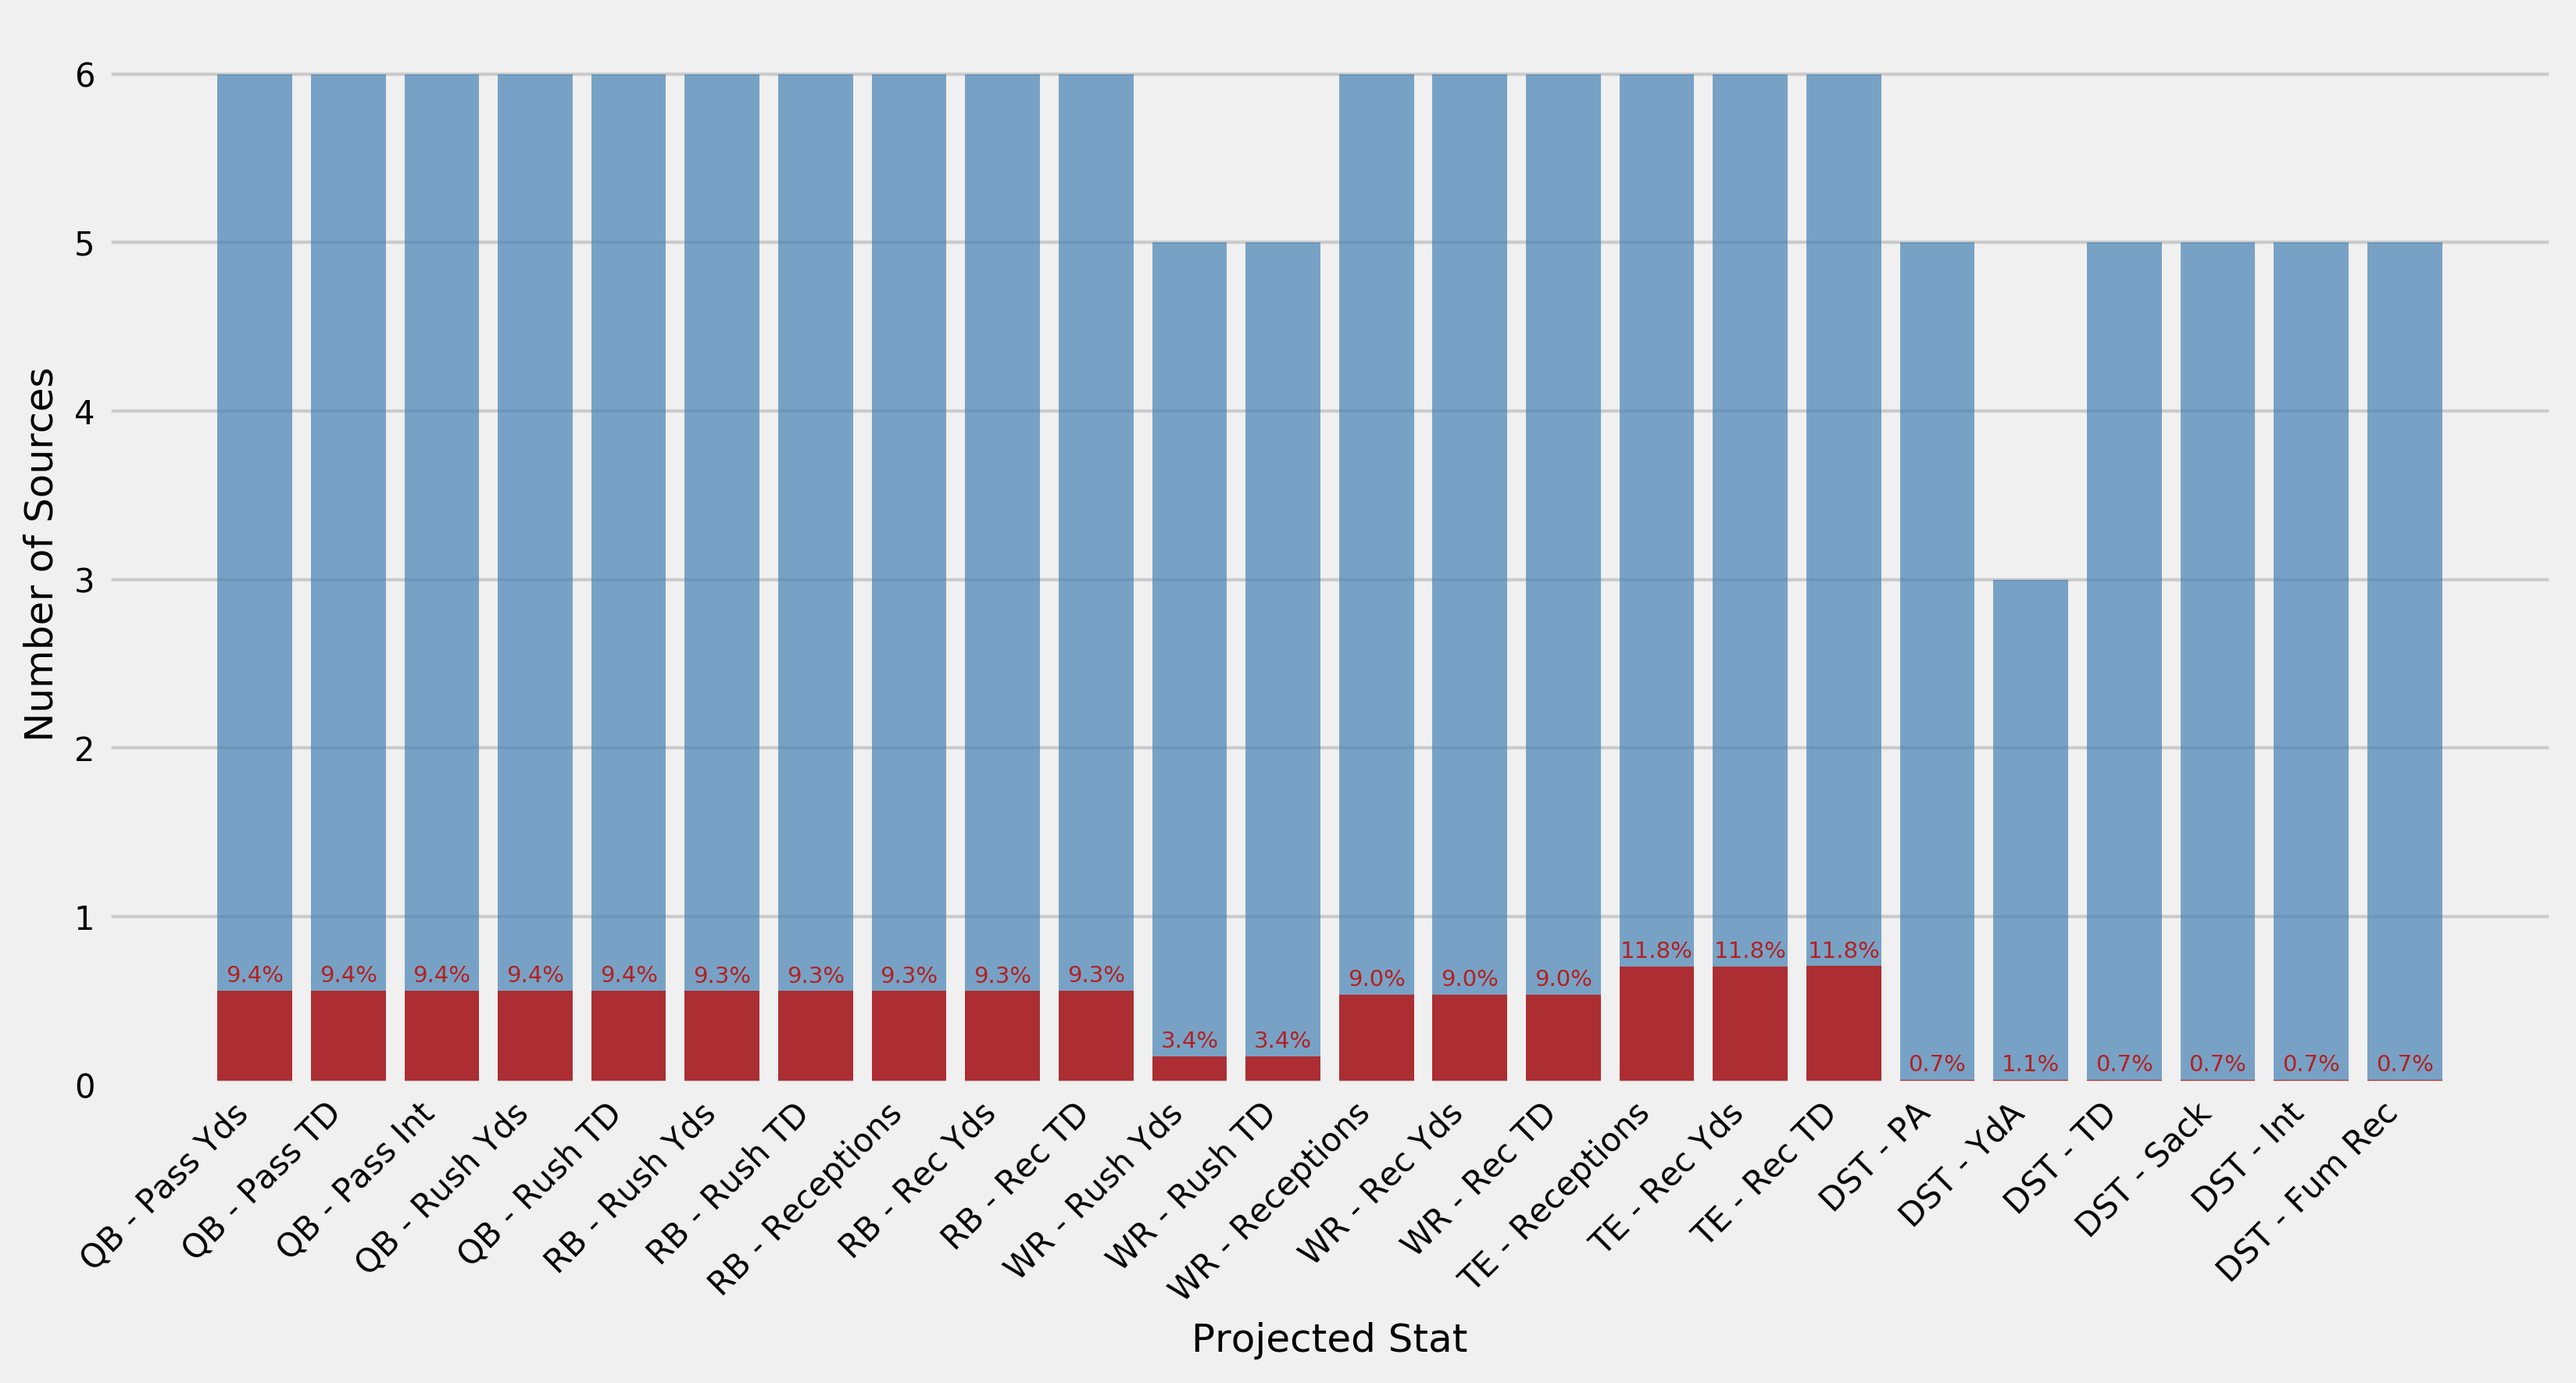
\includegraphics[width=0.95\textwidth]{../figures/missing_data}
  \caption{Number of sources collected for each essential stat (blue). Red indicates percentage of missing data for each respective stat.}
  \label{missing data}
\end{figure}

Several imputing methods were tested to find the optimal method for imputing missing projections. Imputing algorithms from the \texttt{fancyimpute} Python package were utilized to perform the imputing\cite{fancyimpute}. The simplest of these techniques as simply filling the projections from missing sources with the mean or median of the collected projections. Several more advanced methods were also studied. First, an iterative imputing method was used, where each source with missing values was first modeled as a function of all other sources using rows with full data, and these respective models were subsequently used to impute missing values for each source. Second, a K-nearest neighbors (KNN) approach was used, where each source is given a weight based on rows with all data observed. A matrix factorization approach was also studied which uses gradient descent to directly solve a factorization of the incomplete matrix into low-rank $U$ and $V$ matrices with L1 and L2 regularization respectively. Finally a soft impute method was studied which completes the matrix via soft thresholding singular value decompositions (SVD). Strictly using SVD was not possible due to the low number of sources (6) compared to the number of players which ranged from 32 for DST to upwards of 200 for WR. More information regarding each method and literature is available at \cite{fancyimpute}.\bigskip

In order to test which imputing method was best suited for the stat projection dataset, a raw matrix of all projected players for every week of the season was compiled for each stat. Players with 50\% or more sources missing were dropped, as these players were always either backups or players not expected to start, resulting in an incomplete matrix. Next, the percentage of missing data in the incomplete matrix for each respective stat was recorded, shown in Figure \ref{missing data}. All rows (players) with any missing values were subsequently removed, leaving a fully completed matrix for each stat. Elements in this completed matrix were then removed at random until the matrix had an equivalent missing data percentage as incomplete matrix. Each imputation method described above was then used to impute these missing values, with the mean average error (MAE) and root mean squared error (RMSE) recorded for the difference between the imputed matrix of each method and the complete matrix of true projection values. This process was repeated for 50 simulations in order to reduce potential variation from the random selection of missing elements. The resulting MAE and RMSE values for each imputing method of the essential stats is provided below. 


\begin{figure}[H]
  \centering
  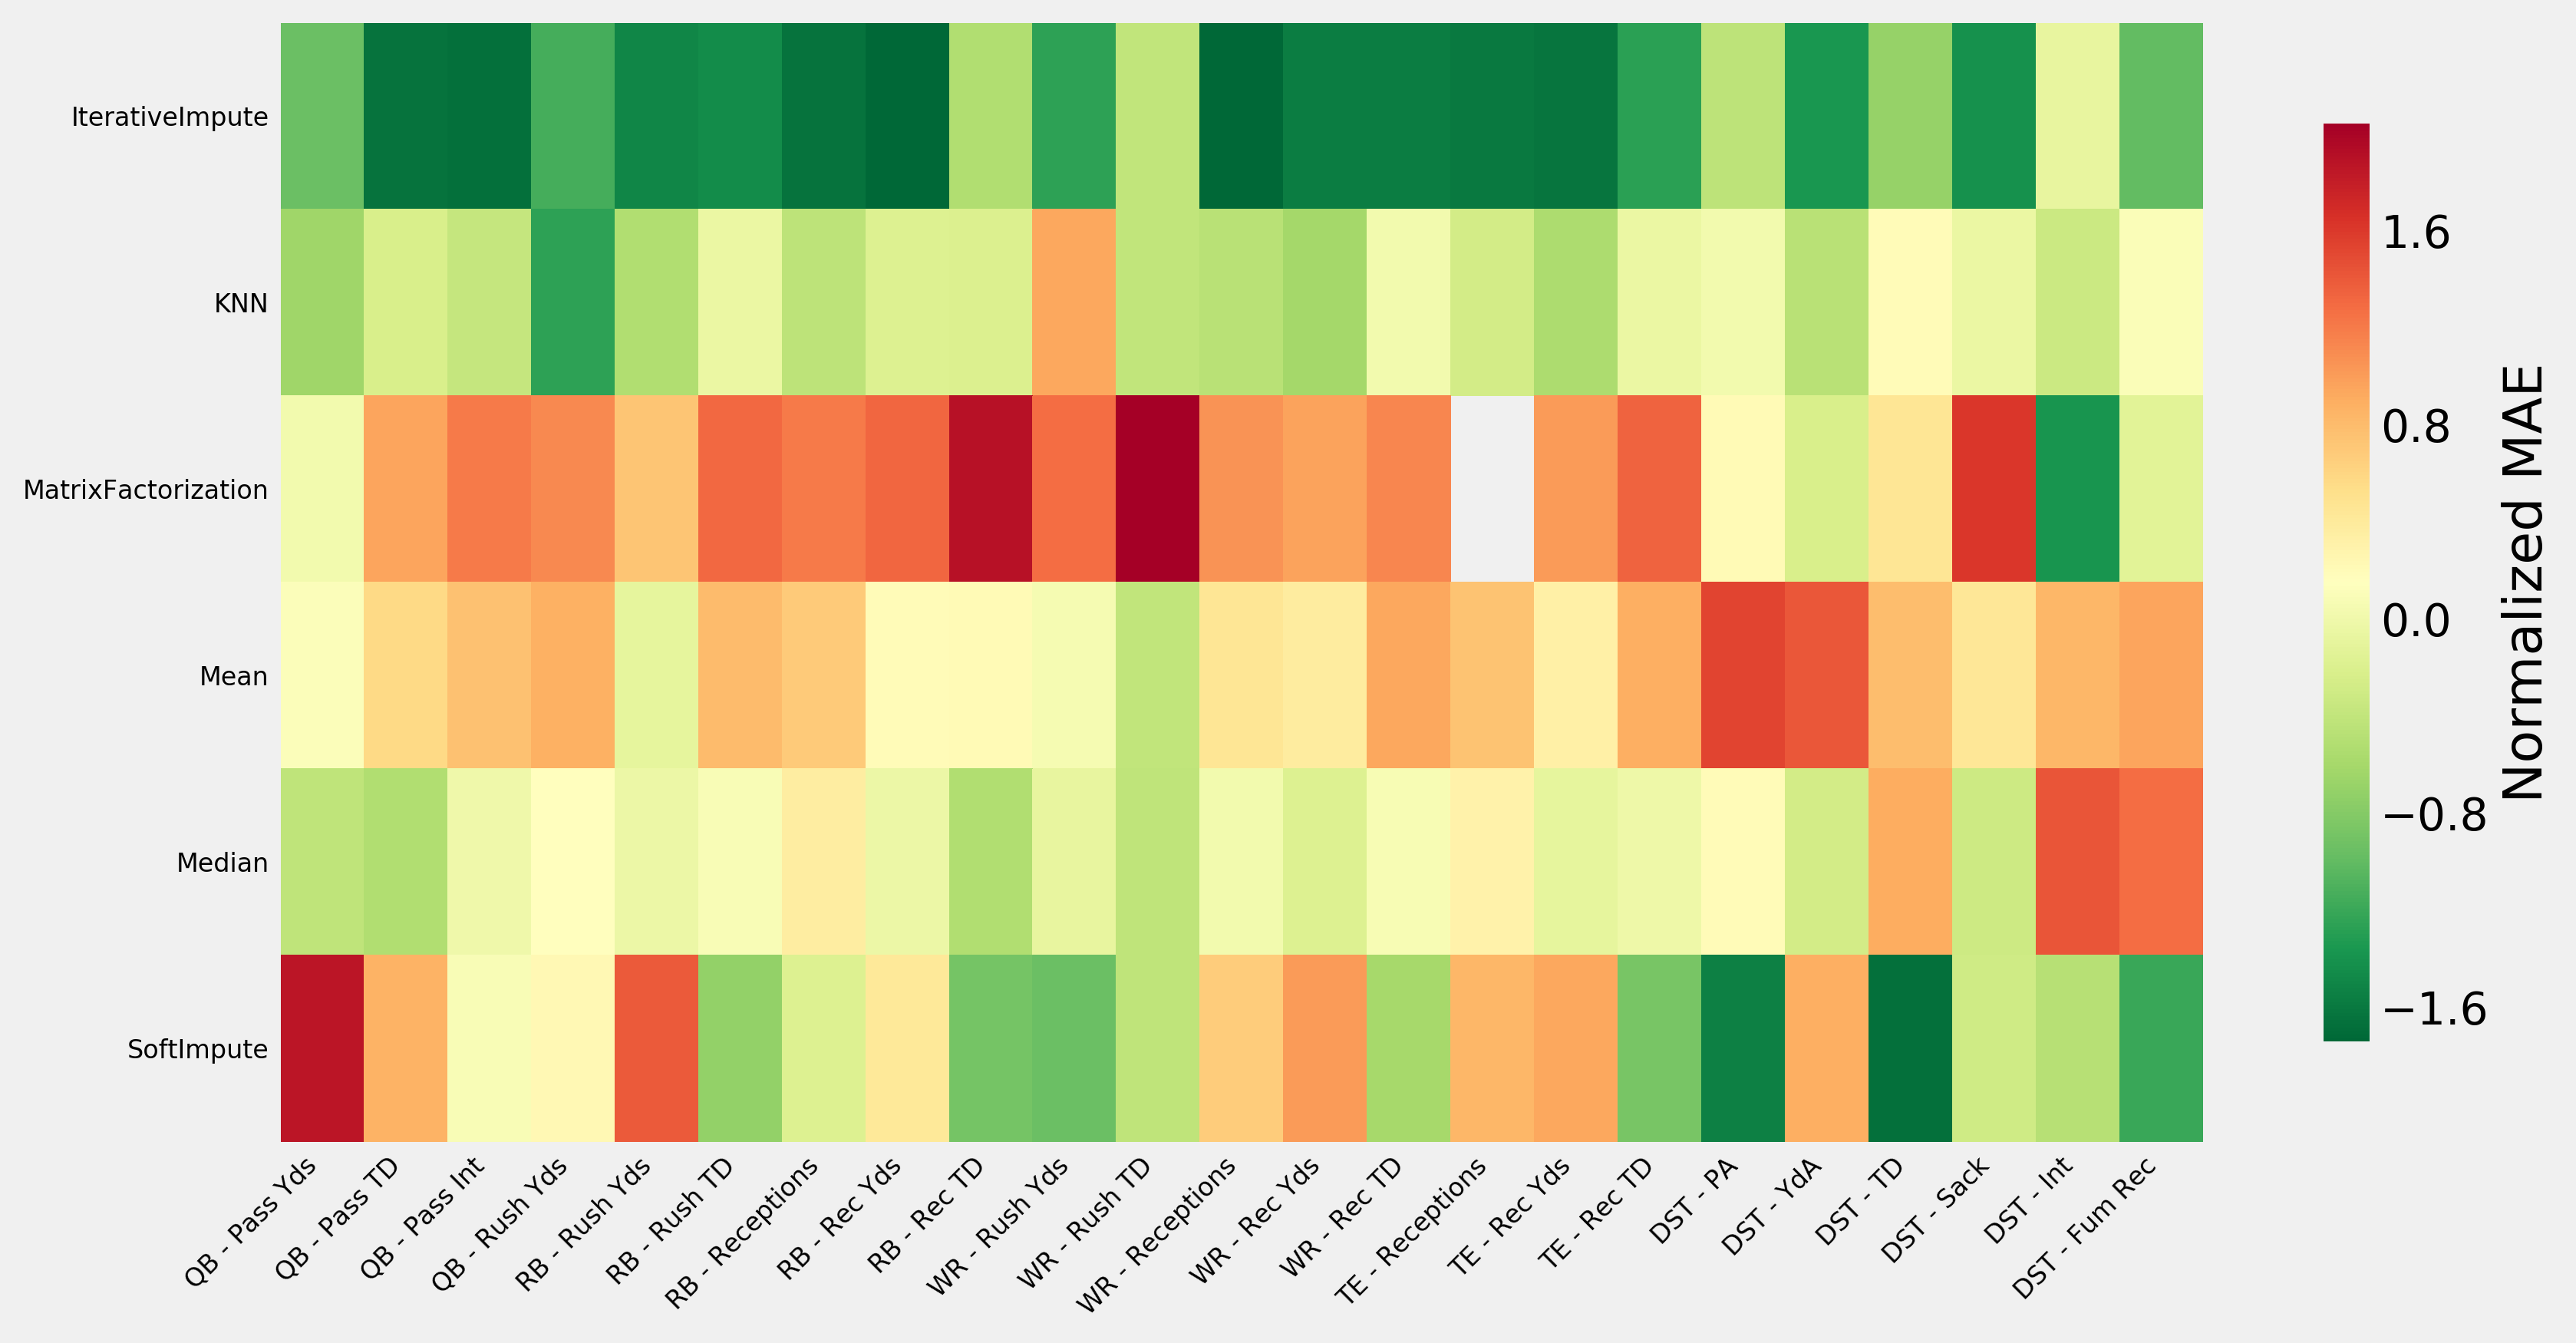
\includegraphics[width=0.95\textwidth]{../figures/impute_MAE}
  \caption{Normalized MAE of imputing methods for each essential stat.}
  \label{impute MAE}
\end{figure}

\begin{figure}[H]
  \centering
  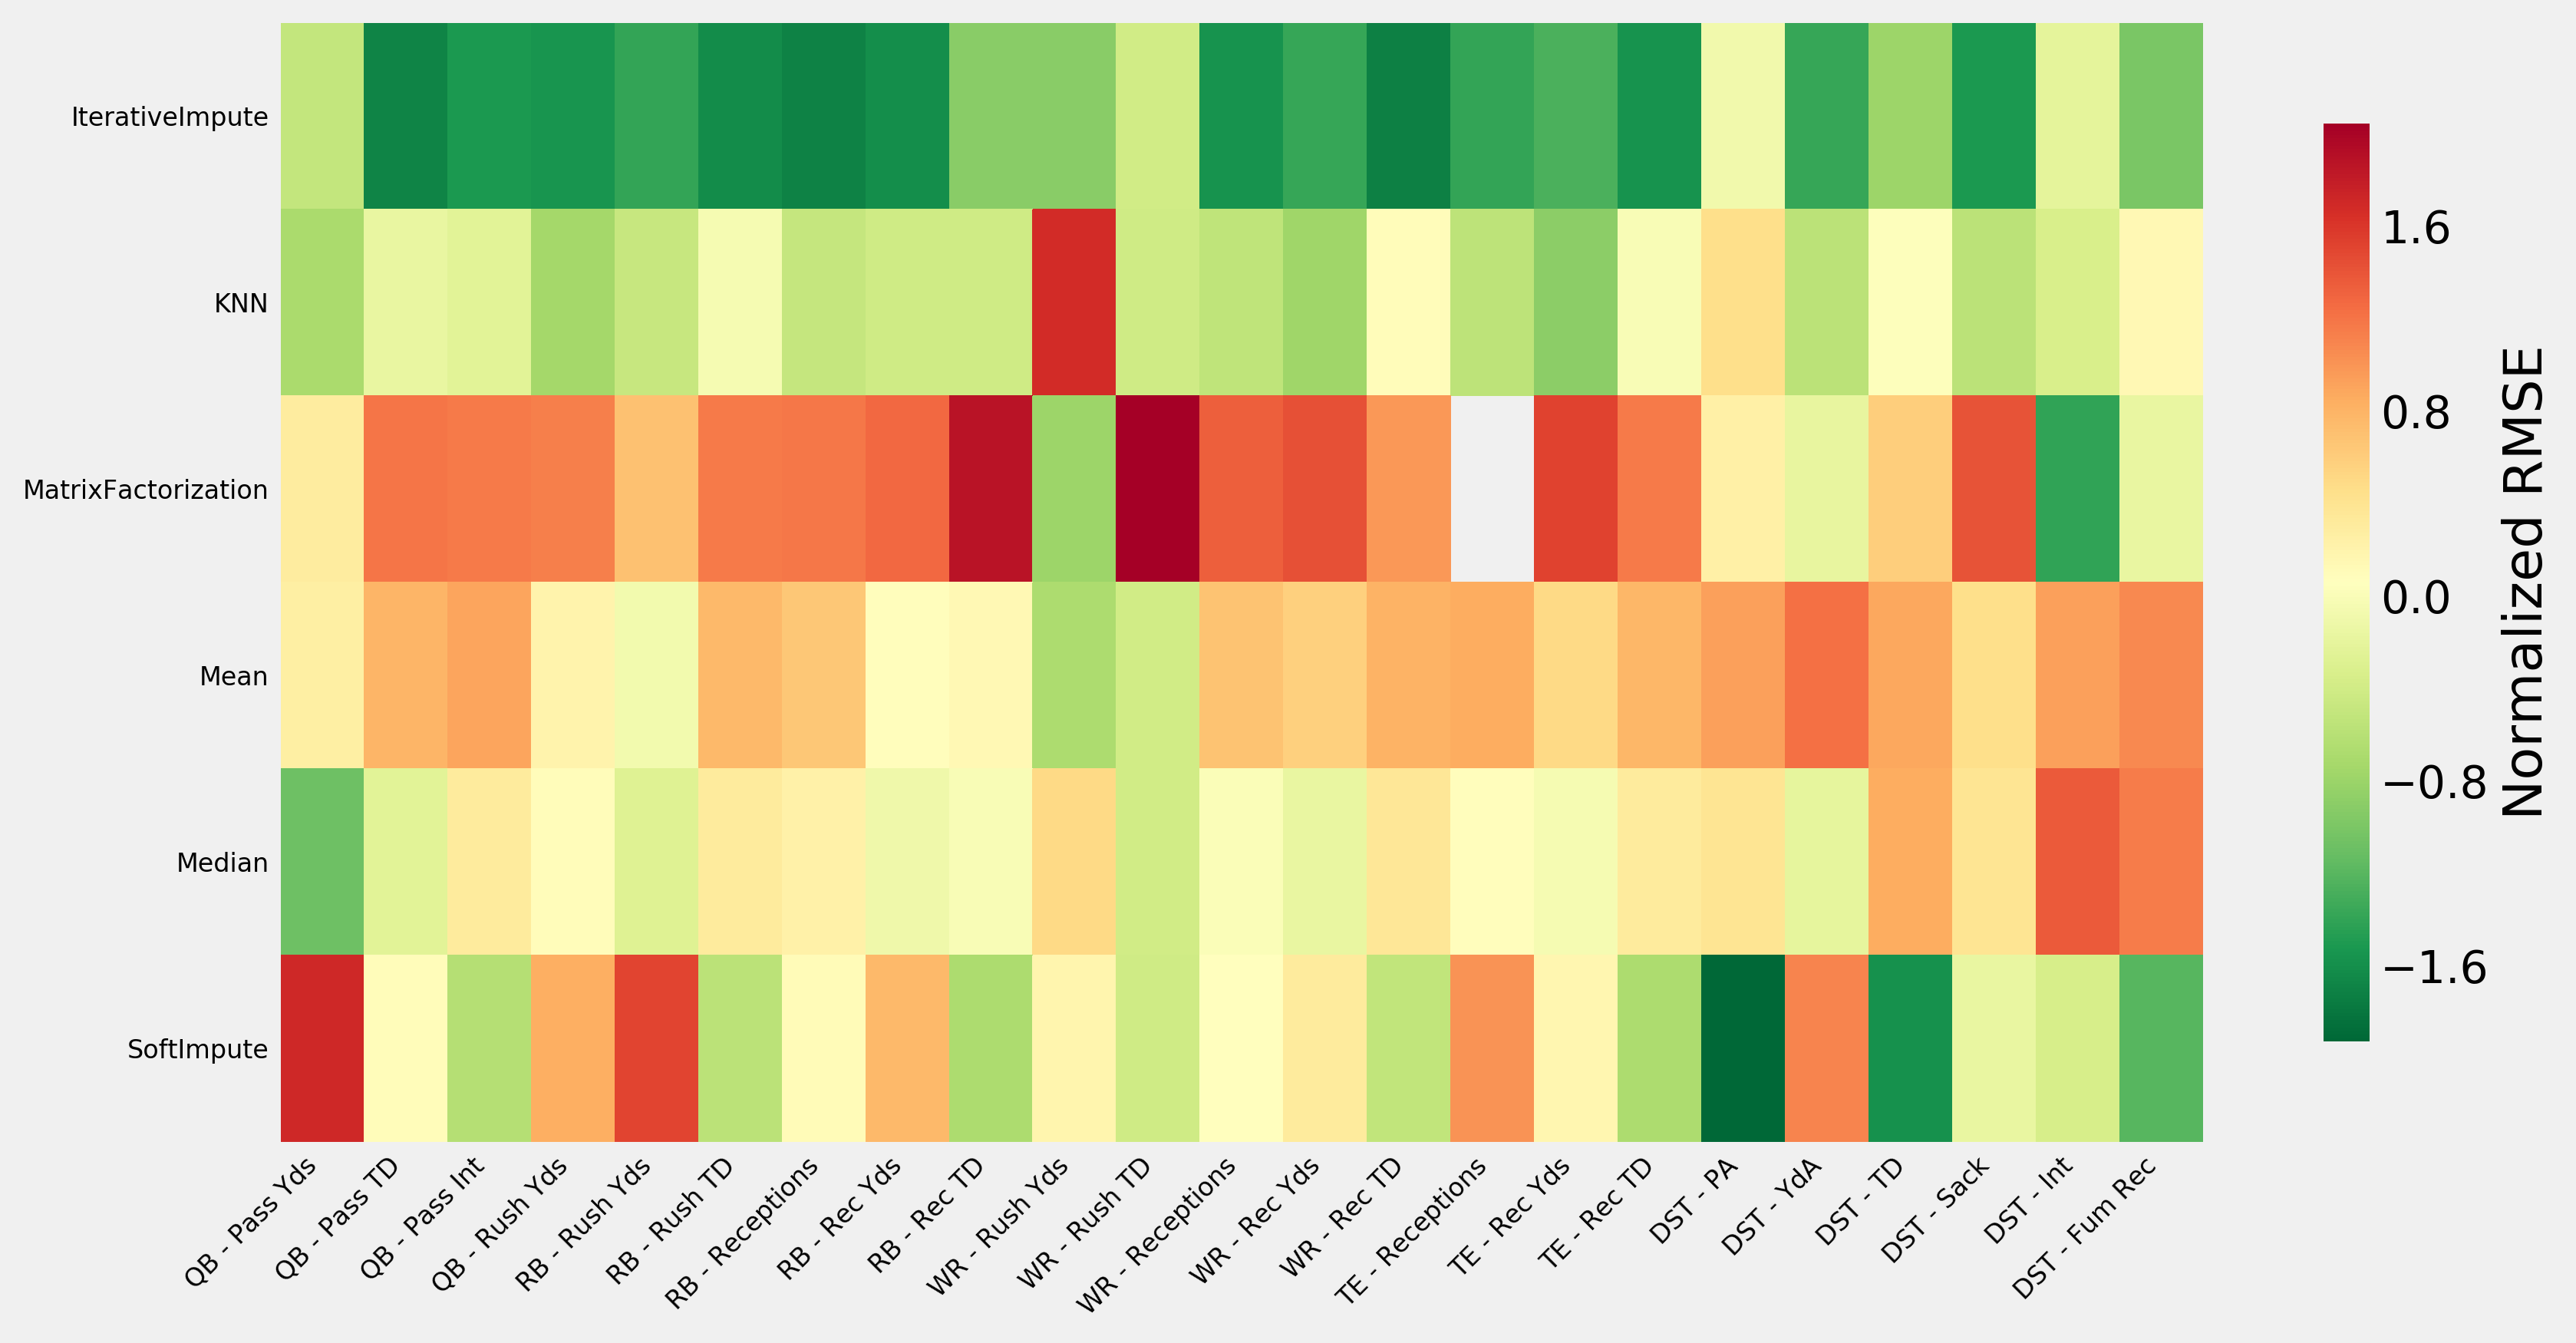
\includegraphics[width=0.95\textwidth]{../figures/impute_RMSE}
  \caption{Normalized RMSE of imputing methods for each essential stat.}
  \label{impute RMSE}
\end{figure}

Figures \ref{impute MAE} and \ref{impute RMSE} clearly indicate that the iterative imputing method provides the best estimates for missing values.  A comparison of imputing techniques for nonessential stats is provided in the appendix, where iterative imputing was again found to be optimal. Therefore iterative imputing was used to impute missing values for both essential and nonessential stats for the remainder of this study.

\subsection{Data Exploration}
TODO

\pagebreak
\section{Methodology}
TODO



\pagebreak
\section{Results}
TODO: 



\pagebreak
\section{Conclusion}
TODO: conclusions

% ------------------------------------ References ---------------------------------------------- %

\pagebreak
\begin{thebibliography}{}

\bibitem{fancyimpute}
A. Rubinsteyn, \& S. Feldman (2019). 
``A Variety of Matrix Completion and Imputation Algorithms Implemented in Python.'' \url{https://github.com/iskandr/fancyimpute}





\end{thebibliography}

\pagebreak
\section{Appendix}
\subsection{Nonessential Stats Summary}

\begin{figure}[H]
  \centering
  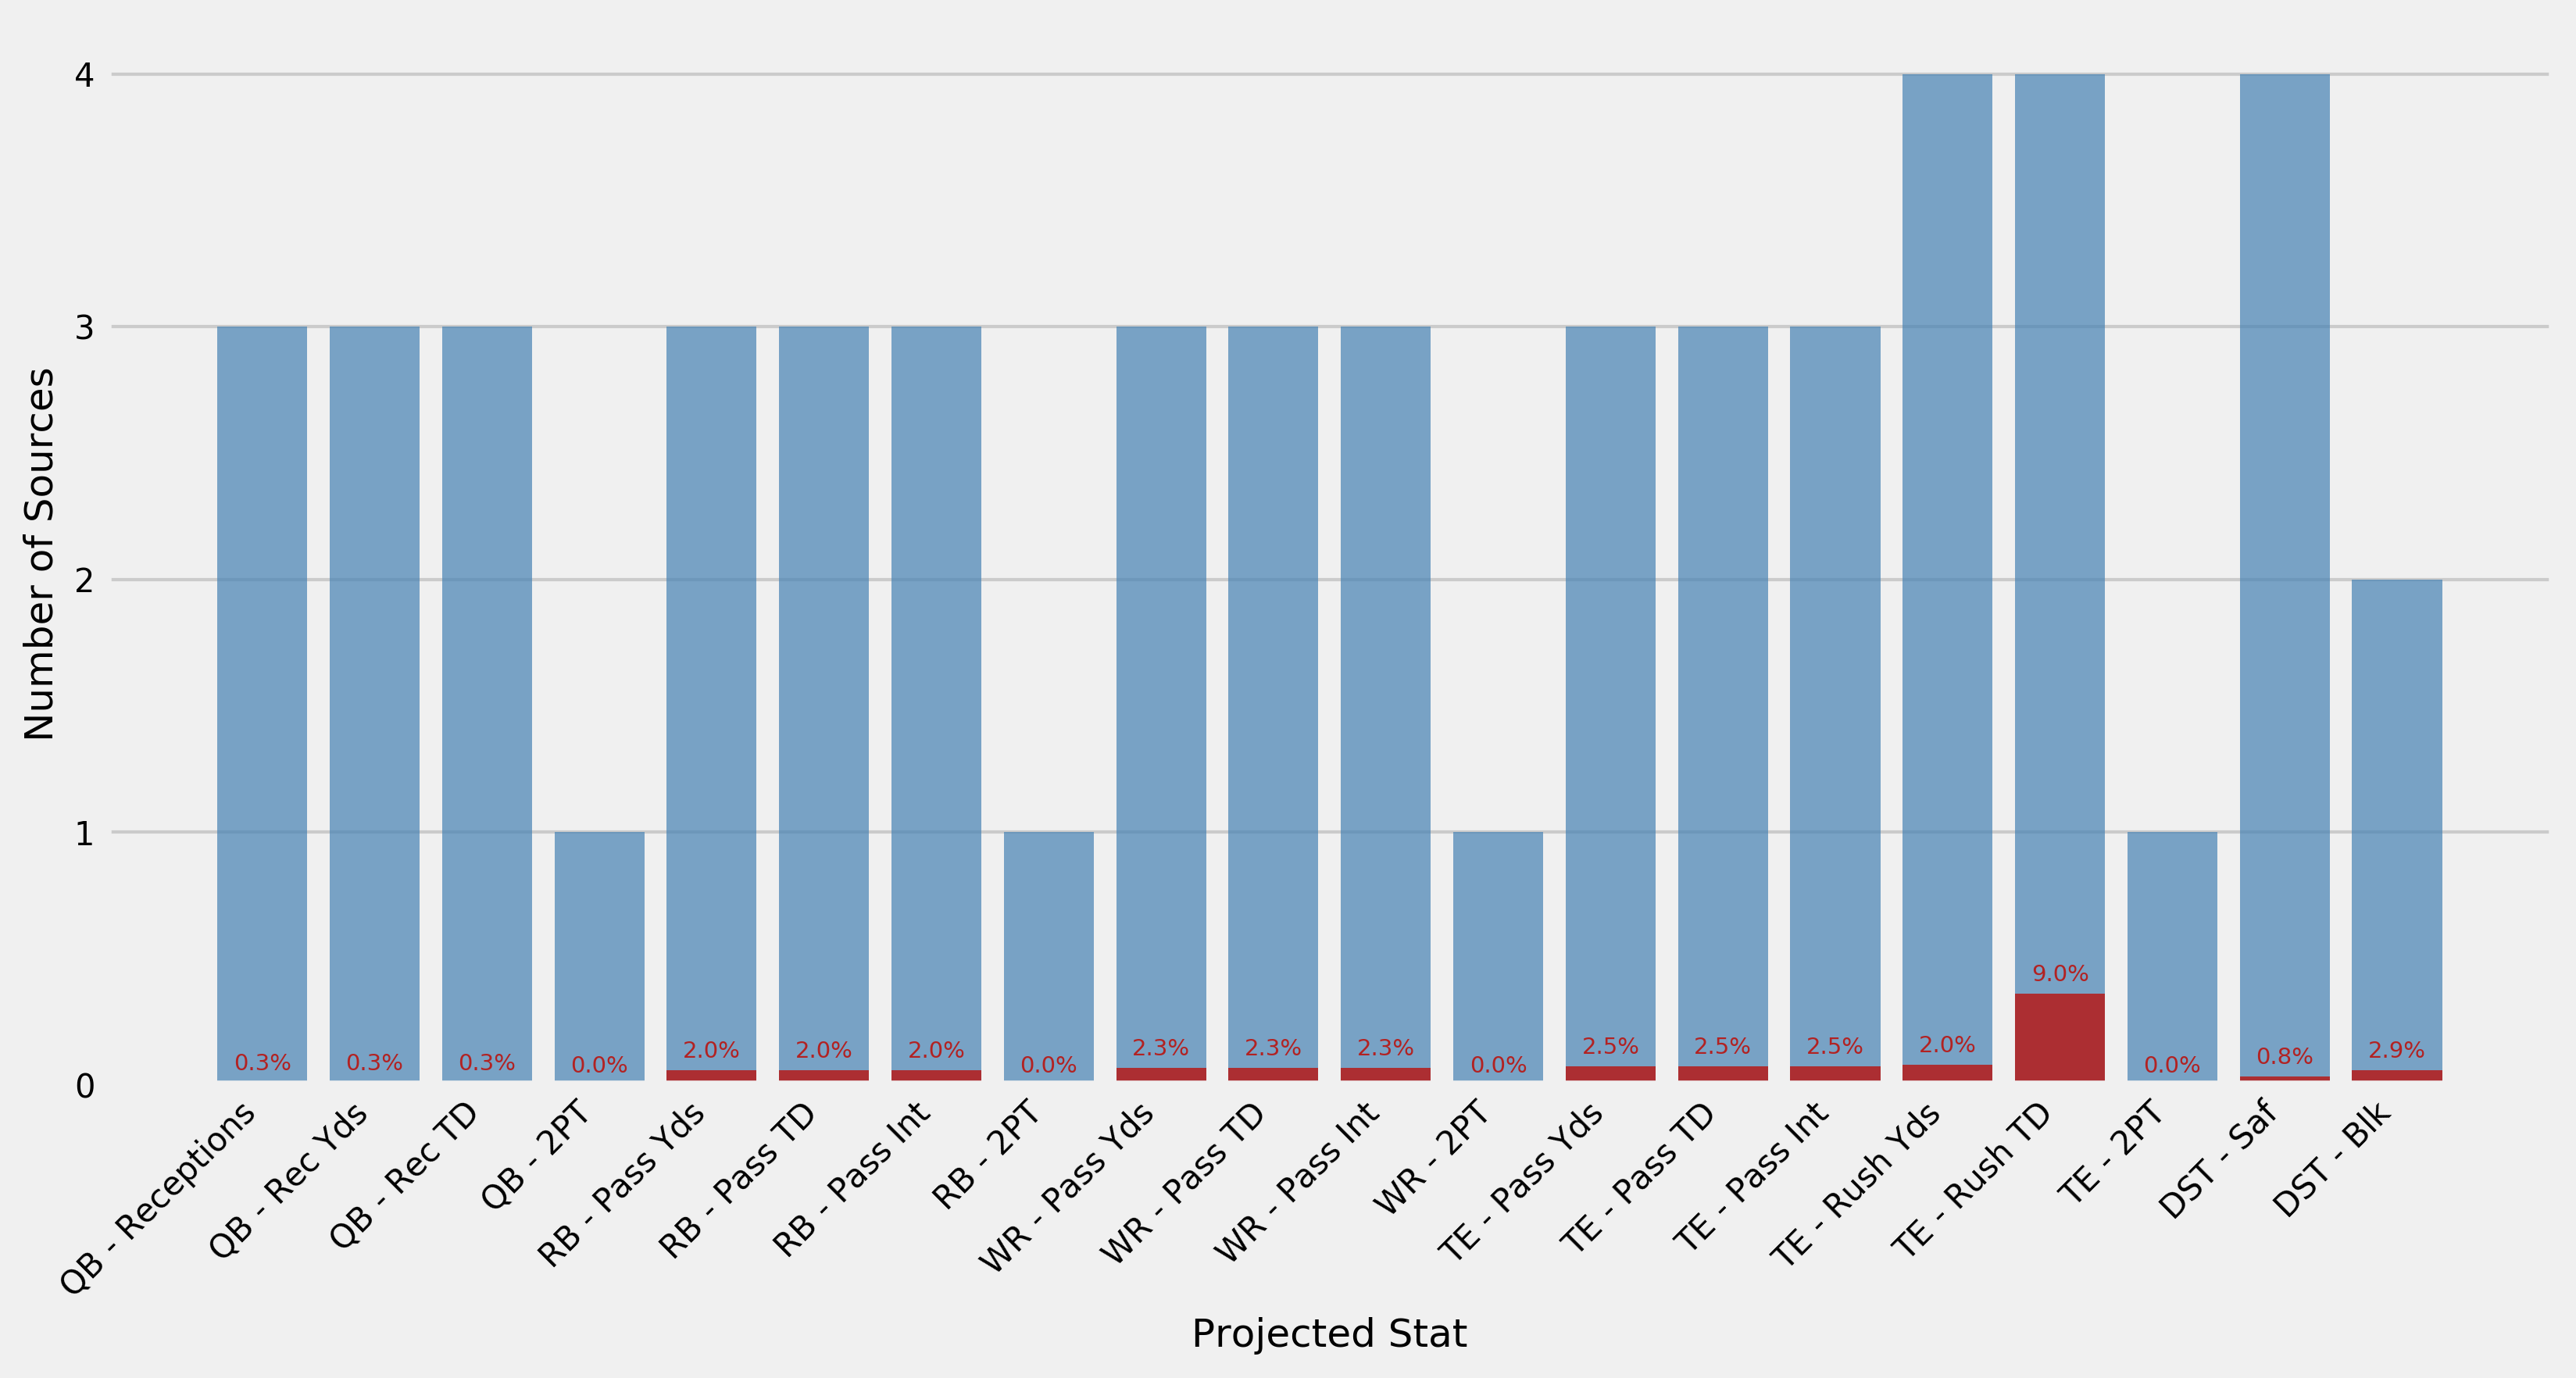
\includegraphics[width=0.95\textwidth]{../figures/nonessential_missing_data}
  \caption{Number of sources collected for each nonessential stat (blue). Red  indicates percentage of missing data for each respective stat.}
\end{figure}

\begin{figure}[H]
  \centering
  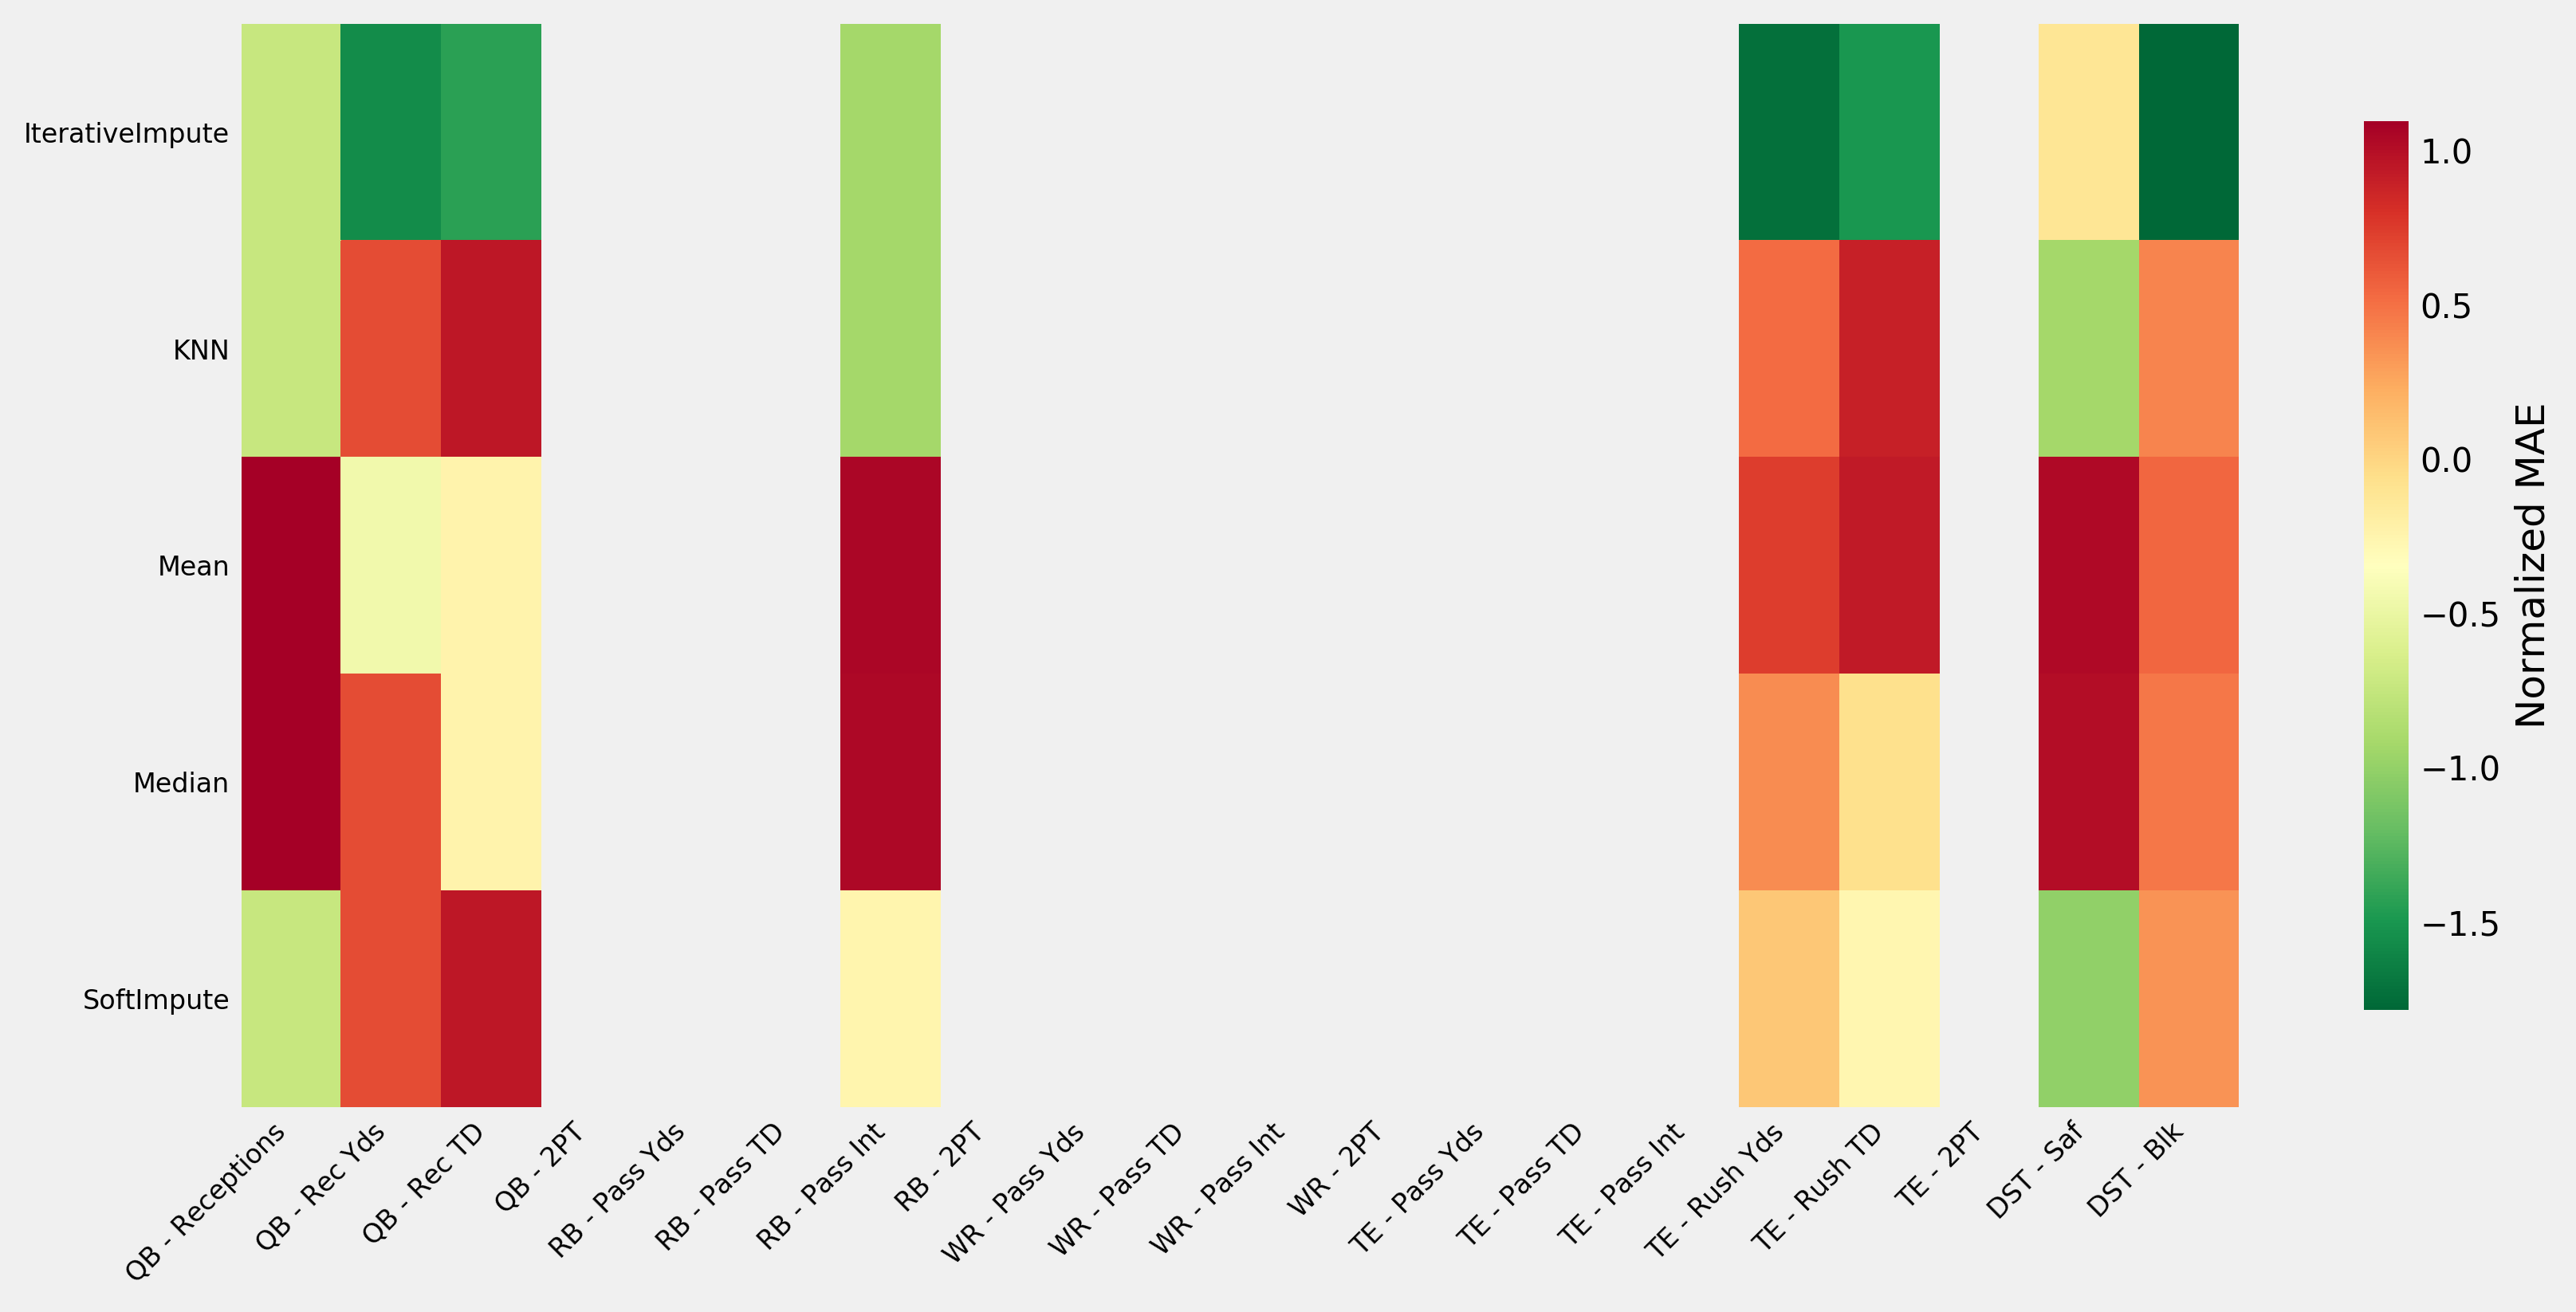
\includegraphics[width=0.95\textwidth]{../figures/nonessential_impute_MAE}
  \caption{Normalized MAE of imputing methods for each nonessential stat.}
\end{figure}

\begin{figure}[H]
  \centering
  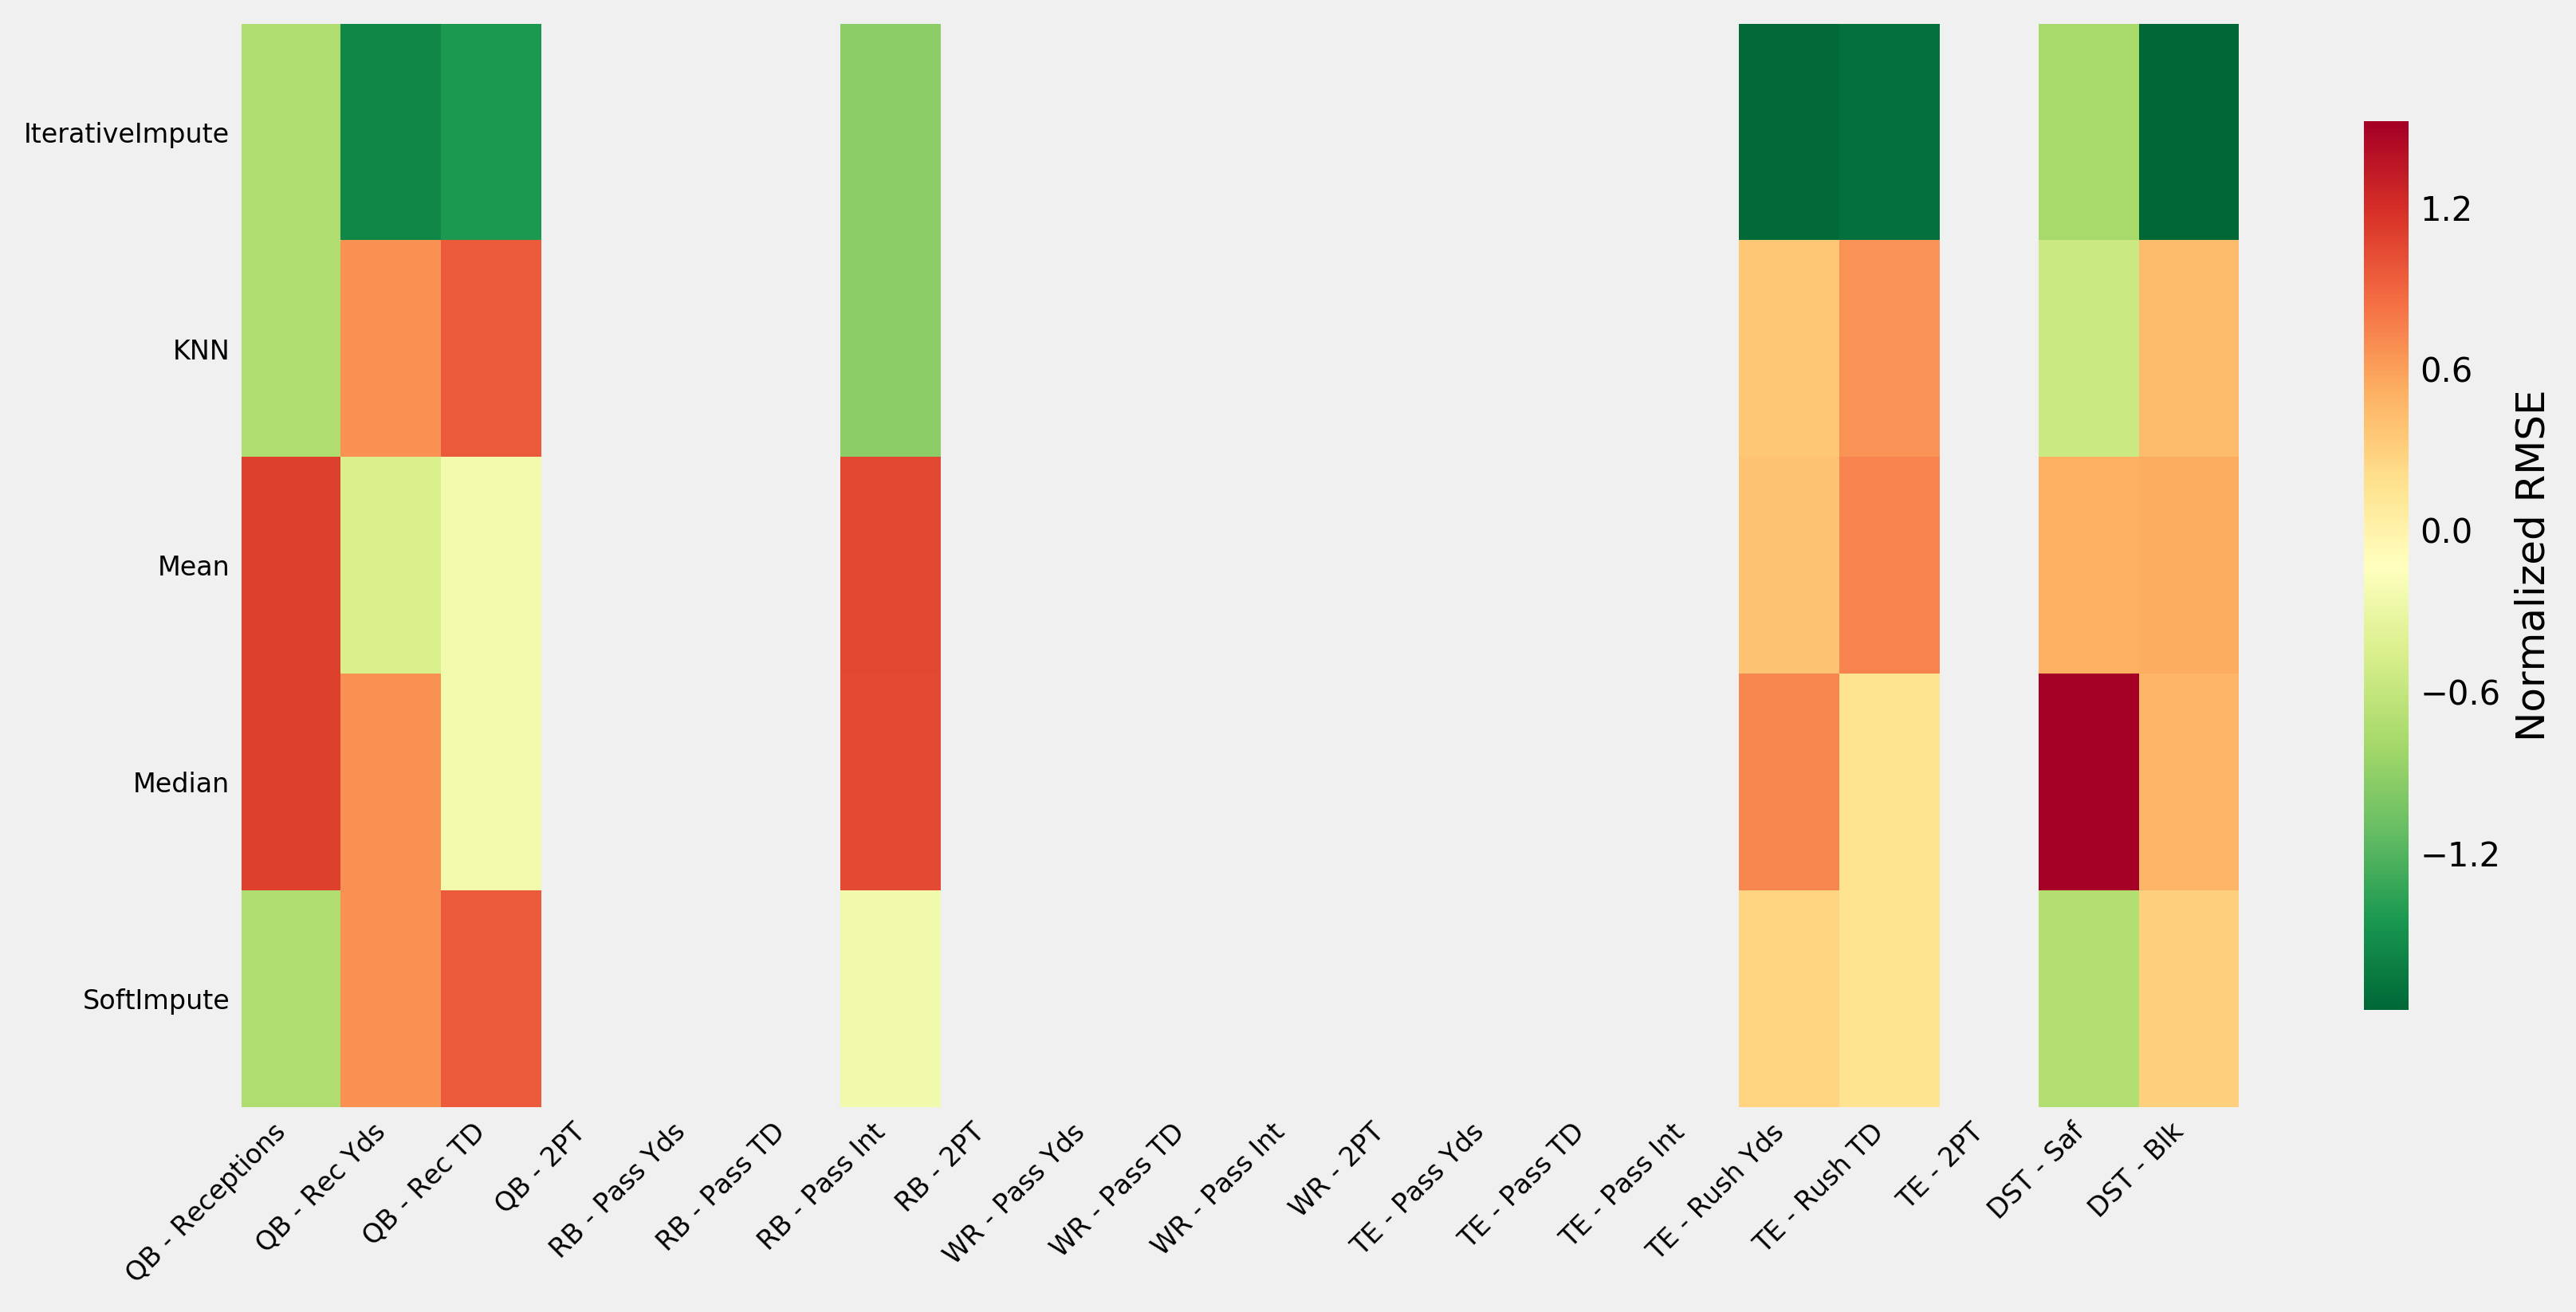
\includegraphics[width=0.95\textwidth]{../figures/nonessential_impute_RMSE}
  \caption{Normalized RMSE of imputing methods for each nonessential stat.}
\end{figure}




\end{document}
